\documentclass[11pt,a4paper]{article}
\usepackage[english]{babel}					% Use english
\usepackage[utf8]{inputenc}					% Caracteres UTF-8
\usepackage{graphicx}						% Imagenes
\usepackage[hidelinks]{hyperref}			% Poner enlaces sin marcarlos en rojo
\usepackage{fancyhdr}						% Modificar encabezados y pies de pagina
\usepackage{float}							% Insertar figuras
\usepackage[textwidth=390pt]{geometry}		% Anchura de la pagina
\usepackage[nottoc]{tocbibind}				% Referencias (no incluir num pagina indice en Indice)
\usepackage{enumitem}						% Permitir enumerate con distintos simbolos
\usepackage[T1]{fontenc}					% Usar textsc en sections
\usepackage{amsmath}						% Símbolos matemáticos
\usepackage{tikz}
\usetikzlibrary{calc}

% Comando para poner el nombre de la asignatura
\newcommand{\subject}{Optimization}
\newcommand{\autor}{Vladislav Nikolov Vasilev}
\newcommand{\titulo}{Optimization Problem 1}
\newcommand{\subtitulo}{Smallest Area problem}
\newcommand{\masters}{Master in Fundamental Principles of Data Science}

\tikzset{
  dot/.style={circle,inner sep=1pt,fill,scale=1.5,label={$#1$},name=#1}
}

\newcommand{\length}[1]{\lvert#1\rvert}
\newcommand{\polyarea}[1]{\left[#1\right]}


% Configuracion de encabezados y pies de pagina
\pagestyle{fancy}
\lhead{\autor{}}
\rhead{\subject{}}
\lfoot{\masters}
\cfoot{}
\rfoot{\thepage}
\renewcommand{\headrulewidth}{0.4pt}		% Linea cabeza de pagina
\renewcommand{\footrulewidth}{0.4pt}		% Linea pie de pagina

\begin{document}
\pagenumbering{gobble}

% Title page
\begin{titlepage}
  \begin{minipage}{\textwidth}
    \centering
    
\includegraphics[scale=0.25]{img/ub-logo}\\[2cm]
    
    \textsc{\Large \subject\\[0.5cm]}
    \textsc{\uppercase\expandafter{\masters}}\\[1.5cm]
    
    \noindent\rule[-1ex]{\textwidth}{1pt}\\[1.5ex]
    \textsc{{\Huge \titulo\\[0.5ex]}}
    \textsc{{\Large \subtitulo\\}}
    \noindent\rule[-1ex]{\textwidth}{2pt}\\[3.5ex]
  \end{minipage}
  
  \vspace{2cm}
  
  \begin{minipage}{\textwidth}
    \centering
    
    
\includegraphics[scale=0.4]{img/ub-ds-logo}
    \vspace{2cm}
    
    \textbf{Author}\\ {\autor{}}\\[2.5ex]
    \textsc{Faculty of Mathematics and Computer Science}\\
    \vspace{1em}
    \textsc{Academic year 2021-2022}
  \end{minipage}
\end{titlepage}

\pagenumbering{arabic}
\setlength{\parskip}{1em}


\section{Problem description}

\emph{\textbf{Given an angle with vertex $A$ and a point $O$ in its interior.
Pass a line $BC$ through the point $O$ that cuts off from the angle a triangle
of minimal area.}}

\begin{center}
  \begin{tikzpicture}
    \node [dot=A] at (0, 0) {};
    \node [dot=O] at (3, 1) {};
    \draw (A) -- (7,0);
    \draw (A) -- (5,4);
  \end{tikzpicture}
\end{center}

\section{Solution}

Let $l$ be the line that passes through the point $O$ and cuts off from the
angle a triangle of minimal area. The intersection points of this line with the angle
are going to be $B$ and $C$. These points will form the segment $BC$ where the
midpoint is going to be $O$.

First, let's name the horizontal line as $p$ and the other one as $q$ so we have an easily
followable naming convention. We obtain the following:

\begin{center}
  \begin{tikzpicture}
    \node [dot=A] at (0, 0) {};
    \node [dot=O] at (3, 1) {};
    
    \draw (A) -- node [below, xshift=60pt] {$p$} (7,0);
    \draw (A) -- node [above, xshift=30pt, yshift=30pt] {$q$} (5,4);
  \end{tikzpicture}
\end{center}

Now, let's try to prove our initial statement. Let $s$ be a symmetry with respect to the
point $O$. If we apply $s$ to $A$, we obtain the point $A' = s(A)$. Now, if we apply $s$ to
the line $p$, we obtain the line $p' = s(p)$. Note that the line $p'$ is parallel to $p$ and
intersects the line $q$ at some point, which we  will call $B$:


\begin{center}
  \begin{tikzpicture}
    \node [dot=A] (A) at (0,0) {};
    \node [dot=O] at (3, 1) {};
    \node [dot=A'] at (6, 2) {};
    
    \node [dot=B] at (2.5, 2) {};
    
    \draw (A) -- node [below, xshift=60pt] {$p$} (7,0);
    \draw (A) -- node [above, xshift=30pt, yshift=30pt] {$q$} (5,4);
    
    \draw [dashed] (A) -- (A');
    \draw (A') -- (-1, 2) node [above, xshift=30pt] {$p'$};
  \end{tikzpicture}
\end{center}

If we pass a line $l$ through $B$ and $O$, it will intersect the line $p$ in a point
named $C$. Note that $C = s(B)$, which means that the point $O$ is the midpoint of the
$BC$ segment and implies that $\length{BO} = \length{OC}$:

\begin{center}
  \begin{tikzpicture}
    \node [dot=A] (A) at (0,0) {};
    \node [dot=O] at (3, 1) {};
    
    \node [dot=A'] at (6, 2) {};    
    \node [dot=B] at (2.5, 2) {};
    \node [dot=C] at (3.5, 0) {};
    
    \draw (A) -- node [below, xshift=60pt] {$p$} (7,0);
    \draw (A) -- node [above, xshift=30pt, yshift=30pt] {$q$} (5,4);
    
    \draw [dashed] (A) -- (A');
    \draw (A') -- (-1, 2) node [above, xshift=30pt] {$p'$};
    \draw [blue] (1.75, 3.5) -- (4.25, -1.5) node [right, yshift=10pt] {$l$};
  \end{tikzpicture}
\end{center}

Next, consider any random line, $r$, which passes through the point $O$. This line
will intersect $q$ and $p$ at some points, $D$ and $E$ respectively:

\begin{center}
  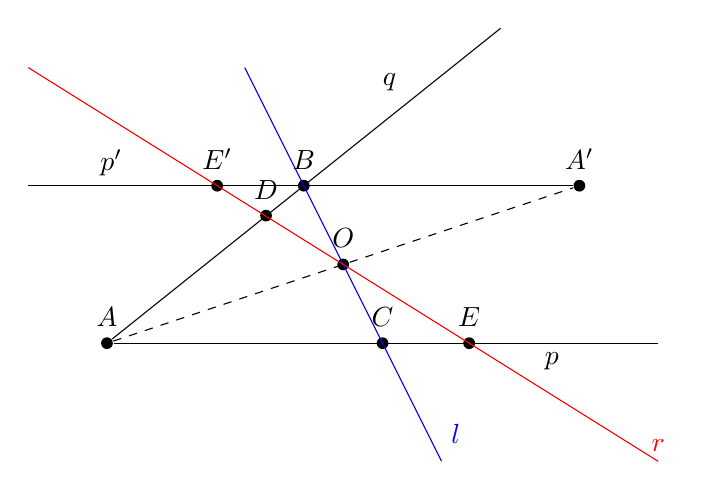
\begin{tikzpicture}
    \node [dot=A] at (0,0) {};
    \node [dot=O] at (3, 1) {};
    
    \node [dot=A'] at (6, 2) {};    
    \node [dot=B] at (2.5, 2) {};
    \node [dot=C] at (3.5, 0) {};
    \node [dot=D] at (2.02, 1.62) {};
    \node [dot=E] at (4.6, 0) {}; 
    \node [dot=E'] at (1.4, 2) {};
    
    \draw (A) -- node [below, xshift=60pt] {$p$} (7,0);
    \draw (A) -- node [above, xshift=30pt, yshift=30pt] {$q$} (5,4);
    
    \draw [dashed] (A) -- (A');
    \draw (A') -- (-1, 2) node [above, xshift=30pt] {$p'$};
    \draw [blue] (1.75, 3.5) -- (4.25, -1.5) node [right, yshift=10pt] {$l$};
    \draw [red] (-1, 3.5) -- (7, -1.5) node [above] {$r$};
  \end{tikzpicture}
\end{center}

Note that in this case $D \neq s(E)$ and instead $E' = s(E)$. This means that the point
$O$ is \textbf{not} the midpoint of the $DE$ segment. Thus, we can easily see that $\length{DO} \neq \length{OE}$.

Now, we have two possible triangles: the triangle $ABC$ and the triangle $ADE$:

\begin{figure}[H]
  \centering
  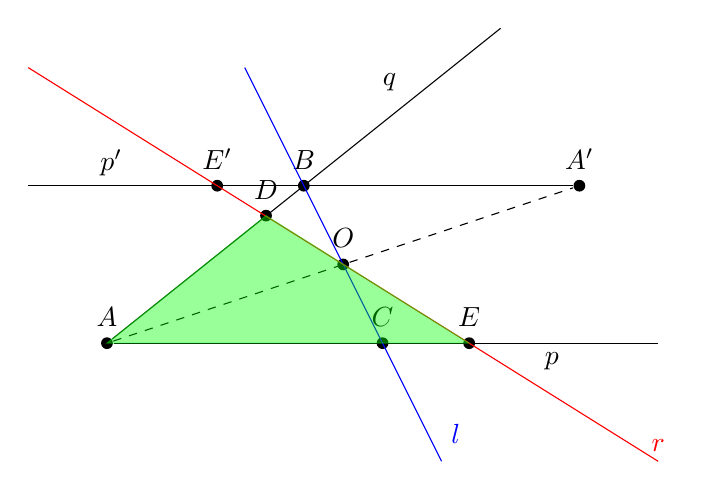
\begin{tikzpicture}
    \node [dot=A] at (0,0) {};
    \node [dot=O] at (3, 1) {};
    
    \node [dot=A'] at (6, 2) {};    
    \node [dot=B] at (2.5, 2) {};
    \node [dot=C] at (3.5, 0) {};
    \node [dot=D] at (2.02, 1.62) {};
    \node [dot=E] at (4.6, 0) {}; 
    \node [dot=E'] at (1.4, 2) {};
    
    \draw (A) -- node [below, xshift=60pt] {$p$} (7,0);
    \draw (A) -- node [above, xshift=30pt, yshift=30pt] {$q$} (5,4);
    
    \draw [dashed] (A) -- (A');
    \draw (A') -- (-1, 2) node [above, xshift=30pt] {$p'$};
    \draw [blue] (1.75, 3.5) -- (4.25, -1.5) node [right, yshift=10pt] {$l$};
    \draw [red] (-1, 3.5) -- (7, -1.5) node [above] {$r$};
    \draw [green, fill=green, opacity=.4] (A.center) -- (D.center) -- (E.center) -- cycle;
  \end{tikzpicture}
  \caption{Representation of the $ADE$ triangle.}
\end{figure}

\begin{figure}[H]
  \centering
  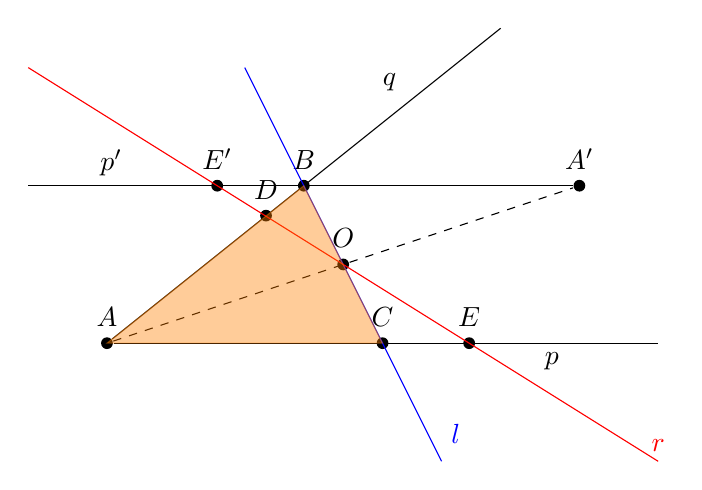
\begin{tikzpicture}
    \node [dot=A] at (0,0) {};
    \node [dot=O] at (3, 1) {};
    
    \node [dot=A'] at (6, 2) {};    
    \node [dot=B] at (2.5, 2) {};
    \node [dot=C] at (3.5, 0) {};
    \node [dot=D] at (2.02, 1.62) {};
    \node [dot=E] at (4.6, 0) {}; 
    \node [dot=E'] at (1.4, 2) {};
    
    \draw (A) -- node [below, xshift=60pt] {$p$} (7,0);
    \draw (A) -- node [above, xshift=30pt, yshift=30pt] {$q$} (5,4);
    
    \draw [dashed] (A) -- (A');
    \draw (A') -- (-1, 2) node [above, xshift=30pt] {$p'$};
    \draw [blue] (1.75, 3.5) -- (4.25, -1.5) node [right, yshift=10pt] {$l$};
    \draw [red] (-1, 3.5) -- (7, -1.5) node [above] {$r$};
    \draw [orange, fill=orange, opacity=.4] (A.center) -- (B.center) -- (C.center) -- cycle;
  \end{tikzpicture}
  \caption{Representation of the $ABC$ triangle.}
\end{figure}

We can easily see that:

$\polyarea{ADE} = \polyarea{ADOC} + \polyarea{OCE} = \polyarea{ADOC} + \polyarea{OBE'} >
\polyarea{ADOC} + \polyarea{DBO} = \polyarea{ABC}$

\noindent which, in short, implies that $\polyarea{ADE} > \polyarea{ABC}$. We can clearly see that
this is due to the fact that $\polyarea{OCE} > \polyarea{DBO}$.

Thus, we can conclude that a line $l$ which intersects with the angle in the points $B$ and $C$
and passes through an interior point $O$ is going to span a triangle with minimal area iif
$B$ and $C$ are equidistant from $O$, or which is the same, the point $O$ is the midpoint of the $BC$
segment.

\end{document}

